\pdfoutput=1
\documentclass[11pt]{article}

\usepackage[T1]{fontenc}
\usepackage[utf8]{inputenc}
\usepackage{lmodern}
\usepackage[margin=1in]{geometry}
\usepackage{microtype}
\usepackage{amsmath}
\usepackage{booktabs}
\usepackage{graphicx}
\usepackage{caption}
\usepackage{subcaption}
\usepackage[numbers,sort&compress]{natbib}
\usepackage[hidelinks]{hyperref}
\usepackage{xurl} % allows line breaks inside long file names and URLs

% generated by paper/make_assets.py from data/ and results/; do not edit
\newcommand{\IQbenchW}{35.6}
\newcommand{\IQbw}{242}
\newcommand{\IQbwPct}{79}
\newcommand{\IQchat}{18.3}
\newcommand{\IQchatGain}{1.58}
\newcommand{\IQchatMTP}{28.9}
\newcommand{\IQfitA}{51.3}
\newcommand{\IQfitB}{0.370}
\newcommand{\IQfitR}{0.988}
\newcommand{\IQheBase}{93.3}
\newcommand{\IQhePlus}{89.6}
\newcommand{\IQjtok}{1.25}
\newcommand{\IQjtokPlain}{1.93}
\newcommand{\IQmtpMax}{1.27}
\newcommand{\IQmtpMin}{1.04}
\newcommand{\IQoverMs}{11.8}
\newcommand{\IQppA}{2.64}
\newcommand{\IQppB}{0.0401}
\newcommand{\IQppLong}{190.0}
\newcommand{\IQppR}{0.991}
\newcommand{\IQppZero}{400.1}
\newcommand{\IQroofMs}{39.5}
\newcommand{\IQsizeGB}{12.12}
\newcommand{\IQtgLong}{13.34}
\newcommand{\IQtgZero}{19.96}
\newcommand{\IQttftLong}{265}
\newcommand{\QEbenchW}{29.4}
\newcommand{\QEbw}{294}
\newcommand{\QEbwPct}{96}
\newcommand{\QEchat}{10.1}
\newcommand{\QEchatGain}{2.24}
\newcommand{\QEchatMTP}{22.6}
\newcommand{\QEfitA}{98.8}
\newcommand{\QEfitB}{0.333}
\newcommand{\QEfitR}{0.9996}
\newcommand{\QEheBase}{92.1}
\newcommand{\QEhePlus}{89.6}
\newcommand{\QEjtok}{1.53}
\newcommand{\QEjtokPlain}{3.33}
\newcommand{\QEmtpMax}{1.75}
\newcommand{\QEmtpMin}{1.32}
\newcommand{\QEoverMs}{4.2}
\newcommand{\QEppA}{2.55}
\newcommand{\QEppB}{0.0410}
\newcommand{\QEppLong}{191.7}
\newcommand{\QEppR}{0.993}
\newcommand{\QEppZero}{414.8}
\newcommand{\QEroofMs}{94.6}
\newcommand{\QEsizeGB}{29.05}
\newcommand{\QEtgLong}{8.28}
\newcommand{\QEtgZero}{10.12}
\newcommand{\QEttftLong}{259}
\newcommand{\cacheMax}{46}
\newcommand{\chatRatioMTP}{1.28}
\newcommand{\concEffIQ}{0.55}
\newcommand{\concEffQE}{0.82}
\newcommand{\hePlusDiffHalfCI}{6.6}
\newcommand{\hePlusK}{147}
\newcommand{\mtpRatioMax}{1.41}
\newcommand{\mtpRatioMin}{1.10}
\newcommand{\ratioPredLong}{1.60}
\newcommand{\ratioPredMax}{1.43}
\newcommand{\sizeRatio}{2.40}
\newcommand{\tgRatioLong}{1.61}
\newcommand{\tgRatioZero}{1.97}


\newcommand{\repo}{\url{https://github.com/eltoncarr/mac-mini-benchmarks}}
\newcommand{\datafile}{\texttt{data/qwen3.8-27b-mac-mini-m5-pro.json}}
% Set to the archived release (tag and DOI) before submission; see SUBMISSION.md.
\newcommand{\datarelease}{v1.0.0}

\title{Bytes per Token Set the Pace:\\ Benchmarking 3.5-bit and 8-bit Qwen3.8-27B\\ on an Apple M5 Pro Mac mini}

\author{%
  Author Name\thanks{Corresponding author: \texttt{author@example.com}. Replace before submission.}\\
  Affiliation
}

\date{October 2026}

\begin{document}
\maketitle

\begin{abstract}
We present a controlled single-machine benchmark of two quantized builds of the dense
Qwen3.8-27B language model running under llama.cpp on an Apple Mac mini with an M5 Pro
system-on-chip (20-core GPU, 64\,GB unified memory, 307\,GB/s): a 3.5-bit-per-weight
GSQ-RCO non-uniform quantization (IQ3\_S, \IQsizeGB\,GB) and a standard 8-bit quantization
(Q8\_0, \QEsizeGB\,GB). Holding hardware, engine version and settings fixed, we measure
decode and prefill throughput across context lengths of 0--64k tokens, the effect of
multi-token-prediction (MTP) speculative decoding, time to first token with and without
prompt caching, concurrent-request throughput, power, and coding accuracy on HumanEval+.
Our thesis is that on this bandwidth-bound unified-memory device, decode speed is set by
the bytes read per token, and the advantage of fewer bytes is bounded by compute headroom.
IQ3\_S decodes \tgRatioZero$\times$ faster than Q8\_0 (\IQtgZero\ vs.\ \QEtgZero\ tokens/s)
with identical HumanEval+ pass@1 (\IQhePlus\%, 95\% confidence interval of the difference
$\pm$\hePlusDiffHalfCI\ points). The advantage narrows to \tgRatioLong$\times$ at 64k
context, where a format-independent attention cost of about 0.35\,ms per token per 1k
tokens of context dominates; it narrows further to \mtpRatioMin--\mtpRatioMax$\times$ with
MTP, because Q8\_0, being memory-bound, has more idle compute for speculative verification
(MTP gain \QEmtpMin--\QEmtpMax$\times$ vs.\ \IQmtpMin--\IQmtpMax$\times$). Prefill is
compute-bound and format-neutral (\IQppZero\ vs.\ \QEppZero\ tokens/s). All measurements,
per-run raw outputs and the benchmark harness are released under open licenses.
\end{abstract}

% ===========================================================================
\section{Introduction}

Unified-memory desktop machines can now hold 20--30\,B-parameter language models at 8-bit
precision, which makes the choice of weight format a practical question for anyone running
models locally: is a much smaller, aggressively quantized file worth it, and what does it
cost? Answering it requires separating three effects that published numbers usually mix:
the hardware's memory bandwidth, the compute cost of a format, and the inference
technique (here, speculative decoding with a multi-token-prediction head).

We study this on one fixed machine, an Apple Mac mini with the M5 Pro chip, with one model,
Qwen3.8-27B~\cite{qwen38card,qwen2025qwen3}, in two builds that bracket the practical range:
ISTA-DASLab's 3.5\,bpw IQ3\_S build produced with GSQ~\cite{dadgarnia2026gsq} and
RCO~\cite{helcig2026rco}, which its authors describe as task-lossless~\cite{istagguf}, and a
conventional Q8\_0 build~\cite{unslothgguf}. Both files carry an MTP head. Everything else
is held constant: llama.cpp commit, server flags, KV-cache type, and measurement tools.

\paragraph{Thesis.} For single-stream decoding on a bandwidth-bound unified-memory device,
throughput is governed by the weight bytes read per generated token. A quality-preserving
3.5-bit format therefore roughly doubles decode speed relative to 8-bit. The advantage is
bounded by the resource the smaller format consumes instead: by shrinking memory traffic,
IQ3\_S moves decoding toward the compute roof~\cite{williams2009roofline}, leaving less idle
compute for speculative decoding and batching to exploit, while context-proportional
attention and compute-bound prefill cost the same in either format.

\paragraph{Contributions.}
\begin{itemize}
  \item A controlled, fully reproducible comparison of IQ3\_S (GSQ-RCO) and Q8\_0 for a dense
        27B model on an M5 Pro, covering decode and prefill over 0--64k tokens of context, MTP,
        prompt caching, concurrency, power and HumanEval+ (Section~\ref{sec:results}).
  \item A two-parameter per-token cost model, fitted per format, that separates weight
        traffic from context cost and accounts for how the speed ratio shrinks with context
        (Section~\ref{sec:context}).
  \item Evidence that MTP and batching gains are inversely related to how close a format
        already is to the compute roof, corroborated by power draw (Sections~\ref{sec:mtp}
        and~\ref{sec:serving}).
  \item An open dataset (one row per measurement, CC BY 4.0) and harness, plus a llama.cpp
        Apple Silicon reference run that places this machine relative to other Macs
        (Section~\ref{sec:ref}).
\end{itemize}

% ===========================================================================
\section{Related Work}

\paragraph{LLM inference on Apple Silicon.}
Several recent studies compare inference engines on Apple hardware.
\citet{rajesh2025production} compare MLX, MLC-LLM, Ollama, llama.cpp and PyTorch MPS on an
M2 Ultra; \citet{barrios2026native} present an MLX-native serving system and report higher
throughput than llama.cpp on an M4 Max; \citet{javat2026silicon} compare consumer NVIDIA and
Apple systems; \citet{zhang2026siliconbench} evaluate nine serving engines on unified-memory
desktops for speed, memory and output fidelity; and \citet{waschkowski2026basert} report
substantially higher prefill throughput than llama.cpp on the M5 Pro by using its GPU
neural accelerators. \citet{kannan2026greenbench} study energy per token on an M4 Pro.
These works vary the engine or the hardware. We hold both fixed and vary the weight format
and the decoding technique, so the differences we report are attributable to them.

\paragraph{Performance models.}
The roofline model~\cite{williams2009roofline} and its application to transformer
inference~\cite{pope2023scaling} explain why autoregressive decoding at batch size one is
bound by memory bandwidth. \citet{bi2026rooflinebench} apply roofline analysis to on-device
LLMs, and \citet{qiu2026ggufmeta} predict single-sequence llama.cpp throughput from GGUF
metadata across Apple and NVIDIA systems. Our per-token cost model is in the same spirit,
fitted per format on one machine, and is used to explain how the format advantage changes
with context length.

\paragraph{Quantization.}
Post-training weight quantization methods such as GPTQ~\cite{frantar2023gptq},
AWQ~\cite{lin2024awq} and AQLM~\cite{egiazarian2024aqlm} trade accuracy for size. GSQ
learns scalar grids with a Gumbel-Softmax relaxation and remains GGUF-compatible
\cite{dadgarnia2026gsq}; RCO allocates per-tensor formats under an exact size budget
\cite{helcig2026rco}. \citet{kurt2026quant} evaluate llama.cpp quantization levels on an 8B
model, measuring quality and CPU throughput. We contribute device-level performance
measurements for a GSQ-RCO build against Q8\_0 on GPU-accelerated unified memory.

\paragraph{Speculative decoding and multi-token prediction.}
Speculative decoding~\cite{leviathan2023speculative,chen2023speculative} verifies several
drafted tokens in one forward pass. Multi-token prediction heads~\cite{gloeckle2024mtp},
used in DeepSeek-V3~\cite{deepseek2024v3}, can serve as the drafter.
\citet{sah2026beneath} profile two-token MTP on a datacenter GPU and attribute its gains to
amortizing repeated execution per generated token. We measure MTP on a bandwidth-bound
consumer device and show that its gain depends on the weight format.

% ===========================================================================
\section{Experimental Setup}
\label{sec:setup}

\paragraph{Hardware.}
Apple Mac mini (Mac17,16) with an M5 Pro: 6 performance and 12 efficiency CPU cores, a
20-core GPU, 64\,GB of unified memory, and 307\,GB/s peak memory bandwidth (Apple
specification). macOS~27.0, default GPU wired-memory limit (48\,GB). The machine was on mains
power with other applications closed.

\paragraph{Models.}
Qwen3.8-27B~\cite{qwen38card} in two GGUF builds:
IQ3\_S-mtp, file \path{Qwen3.8-27B-GSQ-RCO-IQ3_S-mtp.gguf} (\IQsizeGB\,GB, 3.5\,bpw,
GSQ-RCO)~\cite{istagguf}, and Q8\_0, file \path{Qwen3.8-27B-Q8_0.gguf}
(\QEsizeGB\,GB)~\cite{unslothgguf}. Both include the model's MTP head, which llama.cpp uses
for speculative decoding.

\paragraph{Software.}
llama.cpp~\cite{llamacpp} commit \texttt{d4d82d67f} (build b11516) with the Metal backend.
The server ran with \path{-ngl 999 -fa on --jinja} \path{--cache-type-k q8_0}
\path{--cache-type-v q8_0} \path{-c 131072}, one slot, and the model's reasoning mode disabled for throughput tests. MTP
runs added \path{--spec-type draft-mtp} \path{--spec-draft-n-max 2}. We used llama-bench (bundled
with llama.cpp), llama-benchy~0.4.0~\cite{llamabenchy}, EvalPlus~0.3.1~\cite{evalplussoftware}
and macOS \texttt{powermetrics}.

\paragraph{Protocol.}
Each model ran the same fixed suite (\texttt{./run.sh final} in the released
harness~\cite{thisrepo}), one model at a time:
\begin{enumerate}
  \item \emph{Engine throughput}: llama-bench pp512 and tg128 at context depths 0, 4\,096,
        16\,384, 32\,768 and 65\,536 tokens, five repetitions, no speculative decoding.
  \item \emph{Server throughput}: llama-benchy through llama-server's OpenAI-compatible API,
        512- and 2\,048-token prompts with 128 generated tokens at the same depths, three runs
        per point, every request uncached; repeated with MTP; a prefix-cache run at 4k--32k;
        and a concurrency run with 1, 2 and 4 parallel requests (four server slots, MTP off).
  \item \emph{Short-chat latency}: a 256-token streamed answer to a short coding prompt, MTP off
        and on.
  \item \emph{Coding accuracy}: EvalPlus HumanEval and HumanEval+~\cite{chen2021codex,liu2023evalplus},
        164 problems, greedy decoding, reasoning off, MTP on (speculative decoding does not
        change greedy outputs in principle; see Section~\ref{sec:limits}).
  \item \emph{Power}: \texttt{powermetrics} CPU+GPU+ANE power sampled at 1\,Hz throughout the
        llama-bench and server phases.
\end{enumerate}
Reported speeds are tokens per second. Prefill ``at depth $d$'' is the speed of processing
the prompt when $d$ tokens are already in the context.

\paragraph{Statistics.}
llama-bench reports mean and standard deviation over five repetitions; the server suites
report means over three runs. For HumanEval we report Wilson 95\% intervals for each pass
rate and a Wald 95\% interval for the difference in rates. Per-problem outcomes were not
included in the released data, so the difference interval treats the two runs as
independent samples; it is therefore conservative relative to a paired test.

% ===========================================================================
\section{Results}
\label{sec:results}

\subsection{Decode is bandwidth-bound; fewer bytes means faster tokens}

Table~\ref{tab:sweep} lists engine-level throughput. At zero context, IQ3\_S decodes at
\IQtgZero\ tokens/s and Q8\_0 at \QEtgZero\ tokens/s, a ratio of \tgRatioZero$\times$ for a
file-size ratio of \sizeRatio$\times$. Multiplying file size by decode rate gives the
weight traffic each format sustains: \QEbw\,GB/s for Q8\_0 (\QEbwPct\% of the 307\,GB/s peak)
and \IQbw\,GB/s for IQ3\_S (\IQbwPct\%). File size slightly overstates the bytes read per
token, since it includes the embedding table (one row read per token) and, for IQ3\_S, the
MTP head (unused without speculation), so these are upper bounds. Q8\_0 runs essentially at
the bandwidth roof. IQ3\_S does not reach it: unpacking 3-bit codes costs compute, so a
2.4$\times$ reduction in bytes yields a 2.0$\times$ increase in speed.

\begin{table}[t]
  \centering
  \caption{Engine throughput (llama-bench, tokens/s, mean and standard deviation over five
  repetitions) as a function of the number of tokens already in the context.}
  \label{tab:sweep}
  \small
  \begin{tabular}{r rr rr rr rr}
\toprule
 & \multicolumn{4}{c}{prefill, pp512 (tokens/s)} & \multicolumn{4}{c}{decode, tg128 (tokens/s)} \\
\cmidrule(lr){2-5}\cmidrule(lr){6-9}
context & \multicolumn{2}{c}{IQ3\_S-mtp} & \multicolumn{2}{c}{Q8\_0} & \multicolumn{2}{c}{IQ3\_S-mtp} & \multicolumn{2}{c}{Q8\_0} \\
 & mean & s.d. & mean & s.d. & mean & s.d. & mean & s.d. \\
\midrule
0 & 400.13 & 0.13 & 414.75 & 0.29 & 19.96 & 0.08 & 10.12 & 0.01 \\
4\,096 & 339.42 & 1.02 & 352.81 & 1.40 & 19.06 & 0.06 & 9.97 & 0.02 \\
16\,384 & 300.85 & 0.95 & 306.23 & 1.33 & 16.94 & 0.08 & 9.60 & 0.02 \\
32\,768 & 254.87 & 1.84 & 255.81 & 1.02 & 15.69 & 0.25 & 9.14 & 0.02 \\
65\,536 & 190.00 & 3.00 & 191.74 & 2.18 & 13.34 & 0.05 & 8.28 & 0.00 \\
\bottomrule
\end{tabular}

\end{table}

\subsection{Context cost is format-independent}
\label{sec:context}

Figure~\ref{fig:decode} plots decode time per token against context length. A straight line
$t(L) = a + bL$ fits both formats closely ($R^2 = \IQfitR$ for IQ3\_S and \QEfitR\ for
Q8\_0), with intercepts $a = \IQfitA$\,ms and \QEfitA\,ms and slopes $b = \IQfitB$ and
\QEfitB\,ms per 1k tokens of context. The intercept is the weight-traffic cost: reading
the files once at peak bandwidth takes \IQroofMs\,ms and \QEroofMs\,ms, leaving
\IQoverMs\,ms and \QEoverMs\,ms of per-token overhead, larger for IQ3\_S as its
compute-bound unpacking would predict. The slopes, which reflect attention over the KV cache, are
nearly equal, as expected since the KV cache has the same format for both models (F16, the
llama-bench default). The speed ratio therefore shrinks with context: the fitted lines give
\ratioPredLong$\times$ at 64k tokens (an in-sample point; measured \tgRatioLong$\times$) and
extrapolate to \ratioPredMax$\times$ at 128k, which we did not measure.

\begin{figure}[t]
  \centering
  \begin{subfigure}[t]{0.49\linewidth}
    \centering
    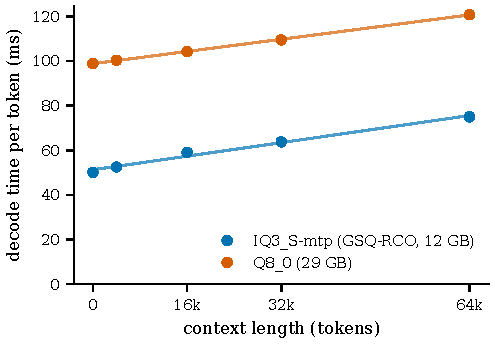
\includegraphics[width=\linewidth]{figures/decode_latency.pdf}
    \caption{Decode time per token with linear fits.}
    \label{fig:decode}
  \end{subfigure}\hfill
  \begin{subfigure}[t]{0.49\linewidth}
    \centering
    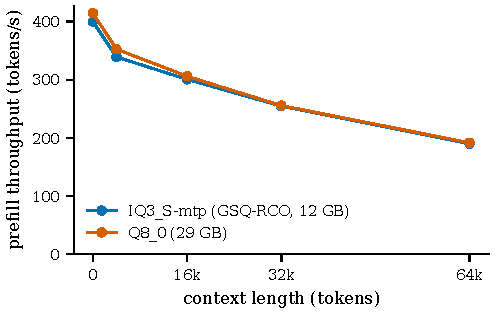
\includegraphics[width=\linewidth]{figures/prefill.pdf}
    \caption{Prefill throughput (pp512).}
    \label{fig:prefill}
  \end{subfigure}
  \caption{Engine-level scaling with context length (llama-bench). Decode cost grows by
  about the same amount per token of context for both formats; prefill is nearly identical.}
\end{figure}

\subsection{Prefill is compute-bound and format-neutral}

Prefill processes many tokens per weight read, so it is limited by compute, not bandwidth.
Both formats prefill at about the same rate (\IQppZero\ vs.\ \QEppZero\ tokens/s at zero
context, \IQppLong\ vs.\ \QEppLong\ at 64k; Figure~\ref{fig:prefill}). Per-token prefill time
again fits a line ($R^2 \geq \IQppR$), with nearly identical intercepts (\IQppA\ and \QEppA\,ms)
and slopes (\IQppB\ and \QEppB\,ms per 1k tokens). The smaller format confers no prefill
advantage. Consequently, a fresh 64k-token prompt takes \IQttftLong\,s (IQ3\_S) and
\QEttftLong\,s (Q8\_0) to its first token (Figure~\ref{fig:ttft}). When the context is already
in llama-server's prompt cache, the first token arrives up to \cacheMax$\times$ sooner (about
2\,s at 32k), which is the regime of multi-turn chat and coding agents. Work on M5 Pro
prefill kernels reports large headroom over llama.cpp~\cite{waschkowski2026basert}, so these
prefill figures are engine-specific.

\subsection{MTP gains depend on compute headroom}
\label{sec:mtp}

Table~\ref{tab:mtp} and Figure~\ref{fig:mtp} compare decoding with and without MTP. MTP
raises Q8\_0's throughput by \QEmtpMin--\QEmtpMax$\times$ on llama-benchy's prose prompts
and by \QEchatGain$\times$ on a short code answer, but IQ3\_S's by only
\IQmtpMin--\IQmtpMax$\times$ and \IQchatGain$\times$. Verifying drafted tokens reads the
weights once for several tokens; it is nearly free when a model waits on memory (Q8\_0) and
costly when compute is already busy (IQ3\_S). With MTP enabled for both, IQ3\_S leads by
\mtpRatioMin--\mtpRatioMax$\times$ over context lengths, and by \chatRatioMTP$\times$ on code
(\IQchatMTP\ vs.\ \QEchatMTP\ tokens/s). The power data in Section~\ref{sec:serving} support
this reading: IQ3\_S draws more power than Q8\_0 during llama-bench (\IQbenchW\ vs.\
\QEbenchW\,W), consistent with higher compute utilization.

\begin{table}[t]
  \centering
  \caption{Decode throughput (tokens/s) through the server API with MTP off and on, after a
  512-token prompt (llama-benchy, mean of three runs). $^\dagger$Short-chat test: a
  256-token streamed answer to a coding prompt.}
  \label{tab:mtp}
  \small
  \begin{tabular}{r rrr rrr r}
\toprule
 & \multicolumn{3}{c}{IQ3\_S-mtp} & \multicolumn{3}{c}{Q8\_0} & IQ3\_S/Q8\_0 \\
\cmidrule(lr){2-4}\cmidrule(lr){5-7}
context & off & MTP & gain & off & MTP & gain & with MTP \\
\midrule
0 & 19.31 & 24.55 & 1.27$\times$ & 10.08 & 17.43 & 1.73$\times$ & 1.41$\times$ \\
4\,096 & 18.58 & 20.21 & 1.09$\times$ & 9.90 & 17.31 & 1.75$\times$ & 1.17$\times$ \\
16\,384 & 16.35 & 19.85 & 1.21$\times$ & 9.46 & 16.02 & 1.69$\times$ & 1.24$\times$ \\
32\,768 & 14.82 & 15.44 & 1.04$\times$ & 8.96 & 14.01 & 1.56$\times$ & 1.10$\times$ \\
65\,536 & 12.68 & 13.58 & 1.07$\times$ & 8.13 & 10.75 & 1.32$\times$ & 1.26$\times$ \\
\midrule
code$^\dagger$ & 18.33 & 28.90 & 1.58$\times$ & 10.09 & 22.64 & 2.24$\times$ & 1.28$\times$ \\
\bottomrule
\end{tabular}

\end{table}

\begin{figure}[t]
  \centering
  \begin{subfigure}[t]{0.49\linewidth}
    \centering
    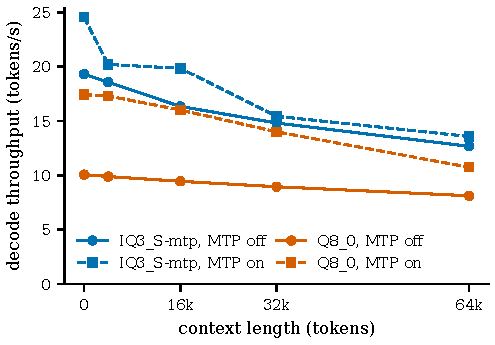
\includegraphics[width=\linewidth]{figures/throughput_mtp.pdf}
    \caption{Decode throughput through the API, MTP off and on.}
    \label{fig:mtp}
  \end{subfigure}\hfill
  \begin{subfigure}[t]{0.49\linewidth}
    \centering
    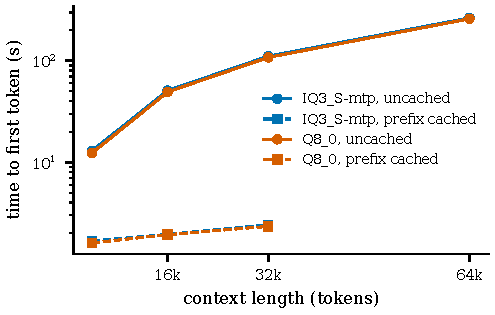
\includegraphics[width=\linewidth]{figures/ttft.pdf}
    \caption{Time to first token for a 512-token prompt.}
    \label{fig:ttft}
  \end{subfigure}
  \caption{Server-level measurements (llama-benchy). Prefix caching applies when the
  existing context is already cached; no cached run was made at 64k.}
\end{figure}

\subsection{No detectable difference in coding accuracy}

Table~\ref{tab:quality} reports HumanEval and HumanEval+ pass@1. Both builds solve
\hePlusK\ of 164 HumanEval+ problems (\IQhePlus\%); on base tests IQ3\_S solves two more.
The 95\% interval for the HumanEval+ difference is $\pm$\hePlusDiffHalfCI\ points, so the
data rule out a large loss from the 3.5-bit format but cannot establish equivalence within
a few points. The evaluation covers short, single-function code generation with reasoning
disabled; it does not measure long-horizon or agentic behaviour.

\begin{table}[t]
  \centering
  \caption{Coding accuracy (EvalPlus, greedy, reasoning off). Wilson 95\% confidence
  intervals, $n = 164$.}
  \label{tab:quality}
  \small
  \begin{tabular}{l rr rr}
\toprule
 & \multicolumn{2}{c}{HumanEval (base tests)} & \multicolumn{2}{c}{HumanEval+ (base + extra)} \\
\cmidrule(lr){2-3}\cmidrule(lr){4-5}
model & pass@1 & 95\% CI & pass@1 & 95\% CI \\
\midrule
IQ3\_S-mtp & 93.3\% (153/164) & [88.4, 96.2] & 89.6\% (147/164) & [84.0, 93.4] \\
Q8\_0 & 92.1\% (151/164) & [86.9, 95.3] & 89.6\% (147/164) & [84.0, 93.4] \\
\bottomrule
\end{tabular}

\end{table}

\subsection{Concurrency and energy}
\label{sec:serving}

Table~\ref{tab:serving} summarizes concurrent-request throughput and power. With four
parallel requests at zero context, total decode throughput is \concEffQE\ of four times the
single-request rate for Q8\_0 but only \concEffIQ\ for IQ3\_S: batching, like MTP,
uses idle compute, and Q8\_0 has more of it. With 4k tokens of context per request, the gain
disappears for both, since other requests' prefill interrupts decoding. Average power while
serving is similar (35.4--36.0\,W vs.\ 33.6--34.7\,W), so energy per generated token follows speed:
\IQjtok\ vs.\ \QEjtok\,J with MTP and \IQjtokPlain\ vs.\ \QEjtokPlain\,J without. These are
whole-phase averages that include prefill, so they are approximate.

\begin{table}[t]
  \centering
  \caption{Concurrency (llama-benchy, 512-token prompts, MTP off) and power
  (\texttt{powermetrics}, CPU+GPU+ANE). $^\ddagger$Server-phase average power divided by
  short-chat decode speed.}
  \label{tab:serving}
  \small
  \begin{tabular}{l rr}
\toprule
measure & IQ3\_S-mtp & Q8\_0 \\
\midrule
total decode, 1 parallel request, 0 context (tokens/s) & 18.7 & 10.1 \\
total decode, 2 parallel requests, 0 context (tokens/s) & 24.0 & 18.2 \\
total decode, 4 parallel requests, 0 context (tokens/s) & 41.0 & 33.1 \\
scaling efficiency at 4 requests, 0 context & 0.55 & 0.82 \\
total decode, 4 parallel requests, 4\,096 context (tokens/s) & 13.6 & 12.6 \\
\midrule
average power, llama-bench (W) & 35.6 & 29.4 \\
average power, server, MTP off (W) & 35.4 & 33.6 \\
average power, server, MTP on (W) & 36.0 & 34.7 \\
energy per generated token, MTP off (J)$^\ddagger$ & 1.93 & 3.33 \\
energy per generated token, MTP on (J)$^\ddagger$ & 1.25 & 1.53 \\
\bottomrule
\end{tabular}

\end{table}

\subsection{Hardware reference}
\label{sec:ref}

To place the machine relative to other Apple systems, we ran the standard Llama-2-7B test of
llama.cpp's Apple Silicon discussion~\cite{llamacpp4167} (llama-bench pp512 and tg128 for
F16, Q8\_0 and Q4\_0, at the commit the thread prescribes, \texttt{c1d0e7a00}). Table~\ref{tab:ref}
compares it with the thread's MacBook Pro entry for the same 20-core M5 Pro: decode agrees
to within 0.8\% and prefill to within 1.7\%. The Mac mini's sustained performance is
therefore representative of the chip, and its cooling did not limit the runs reported here.

\begin{table}[t]
  \centering
  \caption{llama.cpp Apple Silicon reference (Llama-2 7B, tokens/s, commit
  \texttt{c1d0e7a00}).}
  \label{tab:ref}
  \small
  \begin{tabular}{l rr rr rr}
\toprule
 & \multicolumn{2}{c}{F16} & \multicolumn{2}{c}{Q8\_0} & \multicolumn{2}{c}{Q4\_0} \\
\cmidrule(lr){2-3}\cmidrule(lr){4-5}\cmidrule(lr){6-7}
system & pp512 & tg128 & pp512 & tg128 & pp512 & tg128 \\
\midrule
Mac mini, M5 Pro (this work) & 1589.81 & 21.45 & 1579.50 & 38.97 & 1645.99 & 66.84 \\
MacBook Pro, M5 Pro (Discussion \#4167) & 1588.78 & 21.55 & 1553.86 & 38.92 & 1620.64 & 66.33 \\
ratio & 1.001 & 0.995 & 1.017 & 1.001 & 1.016 & 1.008 \\
\bottomrule
\end{tabular}

\end{table}

% ===========================================================================
\section{Discussion}

The measurements support the thesis in four ways. First, decode speed tracks bytes per
token: the format with 2.4$\times$ fewer bytes is 2.0$\times$ faster, and the 8-bit format
runs at 96\% of the bandwidth roof. Second, the cost that does not depend on the format,
attention over the context, is additive and has nearly the same slope for both, so the
advantage decays with context as a two-parameter linear model describes ($R^2 \geq 0.988$). Third,
techniques that convert idle compute into throughput, namely MTP verification and batching,
help the memory-bound 8-bit format more, which narrows but does not close the gap. Fourth,
prefill is compute-bound and identical for both formats, so for long fresh prompts neither
format helps and the engine's compute efficiency dominates.

For practitioners on this class of hardware, the 3.5-bit GSQ-RCO build is the better
operating point on every measure except prefill, where it is 3--4\% slower: it is
2.4$\times$ smaller, 1.1--2.0$\times$ faster in decoding depending on context and MTP, uses about 18\% less energy per token with
MTP, and showed no detectable accuracy loss on HumanEval+. The benefit is smallest exactly
where speculative decoding and long contexts are in use, and prefill performance, not
the weight format, is the next bottleneck for long-context agent workloads.

% ===========================================================================
\section{Limitations}
\label{sec:limits}

\begin{itemize}
  \item \emph{One machine, one model, one engine version.} Results may not transfer to other
        chips, models (in particular mixture-of-experts models with different active-parameter
        ratios~\cite{qiu2026ggufmeta}) or llama.cpp versions; Metal kernels and MTP support
        change frequently.
  \item \emph{Single runs per suite.} llama-bench repeats each test five times (standard
        deviation at most 1.6\% of the mean); the server suites ran
        three times per point and the full protocol once per model.
  \item \emph{Quality.} HumanEval+ is a single greedy run of 164 short problems with reasoning
        disabled. MTP was enabled during this evaluation; speculative decoding preserves the
        target model's output distribution, but floating-point differences between batched and
        unbatched evaluation can change individual greedy tokens. Agentic coding quality was not
        measured at a scale that would separate the two builds.
  \item \emph{Bandwidth estimates} use file size as a proxy for bytes read per token and the
        manufacturer's peak bandwidth; both are approximations.
  \item \emph{Energy} is derived from whole-phase average power, not per-request measurements.
\end{itemize}

% ===========================================================================
\section{Conclusion}

On a 64\,GB Apple M5 Pro running llama.cpp, a 3.5-bit GSQ-RCO build of Qwen3.8-27B decodes
\tgRatioZero$\times$ faster than Q8\_0 at short context and \tgRatioLong$\times$ at 64k, with no
detectable difference on HumanEval+; with MTP the lead is \mtpRatioMin--\mtpRatioMax$\times$.
The pattern follows from a simple account: decode cost is weight traffic plus a
format-independent context term, and speculative decoding and batching profit from whatever
compute the format leaves idle. Benchmarks that report a single tokens-per-second figure
hide these trade-offs; reporting decode across context lengths, with and without
speculation, alongside prefill, makes formats comparable across devices.

% ===========================================================================
\section*{Data and Code Availability}

All results in this paper are generated from the released data by
\texttt{paper/make\_assets.py}. The data are in \datafile\ (one row per measurement with
model, metric, context and prompt length, concurrency, MTP flag, value, unit and tool; a CSV
with the same rows is alongside) and in the per-run folders under \texttt{results/}, which
contain the raw llama-bench, llama-benchy and EvalPlus outputs and the recorded environment.
The benchmark harness (\texttt{bootstrap.sh}, \texttt{run.sh}, \texttt{bench/}) reproduces
every run. Repository: \repo, release \datarelease. Code is MIT-licensed; data and results
are licensed under CC BY 4.0.

\section*{Acknowledgments}

% Edit to reflect your actual use of AI tools; arXiv requires authors to take full
% responsibility for all content and does not allow AI tools as authors.
Portions of the benchmark harness and of this manuscript were drafted with the assistance
of an AI coding assistant. The author ran all measurements, verified the analysis against
the released data, and takes full responsibility for the content.

\bibliographystyle{plainnat}
\bibliography{references}

% ===========================================================================
\appendix
\section{Reproducing the Measurements}

On an Apple Silicon Mac with the repository checked out:
\begin{verbatim}
./bootstrap.sh              # llama.cpp, Python env, models, tokenizer
./run.sh final              # IQ3_S-mtp: llama-bench, server, HumanEval+
MODEL=q8_0 ./run.sh final   # Q8_0
./run.sh ref4167            # llama.cpp Apple Silicon reference
python bench/export.py --out data/qwen3.8-27b-mac-mini-m5-pro \
    results/<IQ3_S run> results/<Q8_0 run> \
    --ref4167 results/<ref4167 run>
python paper/make_assets.py # figures and tables for this paper
\end{verbatim}
The harness records the llama.cpp commit, package versions and hardware in each run's
\texttt{env.json}; \texttt{./run.sh compare} warns if two runs used different commits.

\end{document}
